\documentclass{beamer}
\usepackage{ulem}
\usepackage{amsmath}
\usepackage{amssymb}
\usepackage{subcaption}
\usepackage{graphicx}

\mode<presentation>
{
  \usetheme{metropolis}
}


\usepackage[german]{babel}
% or whatever

\usepackage[utf8]{inputenc}
% or whatever

\setbeamersize{text margin left=1.5em,text margin right=1.5em}

\title{Masterprojekt SS17 -- Dr. Haskell}


\author[shortname]{\centering
	Niels Bunkenburg \and Jonas Busse \and Janina Harms \\
	\and Jan-Hendrik Matthes \and Marc André Wittorf}

\institute{ 
	Arbeitsgruppe für Programmiersprachen und Übersetzerkonstruktion \par
	Institut für Informatik \par
	Christian-Albrechts-Universität zu Kiel}

\date[Short Occasion]{\vfill\centering\today}

\begin{document}
\begin{frame}
	\titlepage
\end{frame}
\begin{frame}
	\frametitle{Softwarearchitektur}
	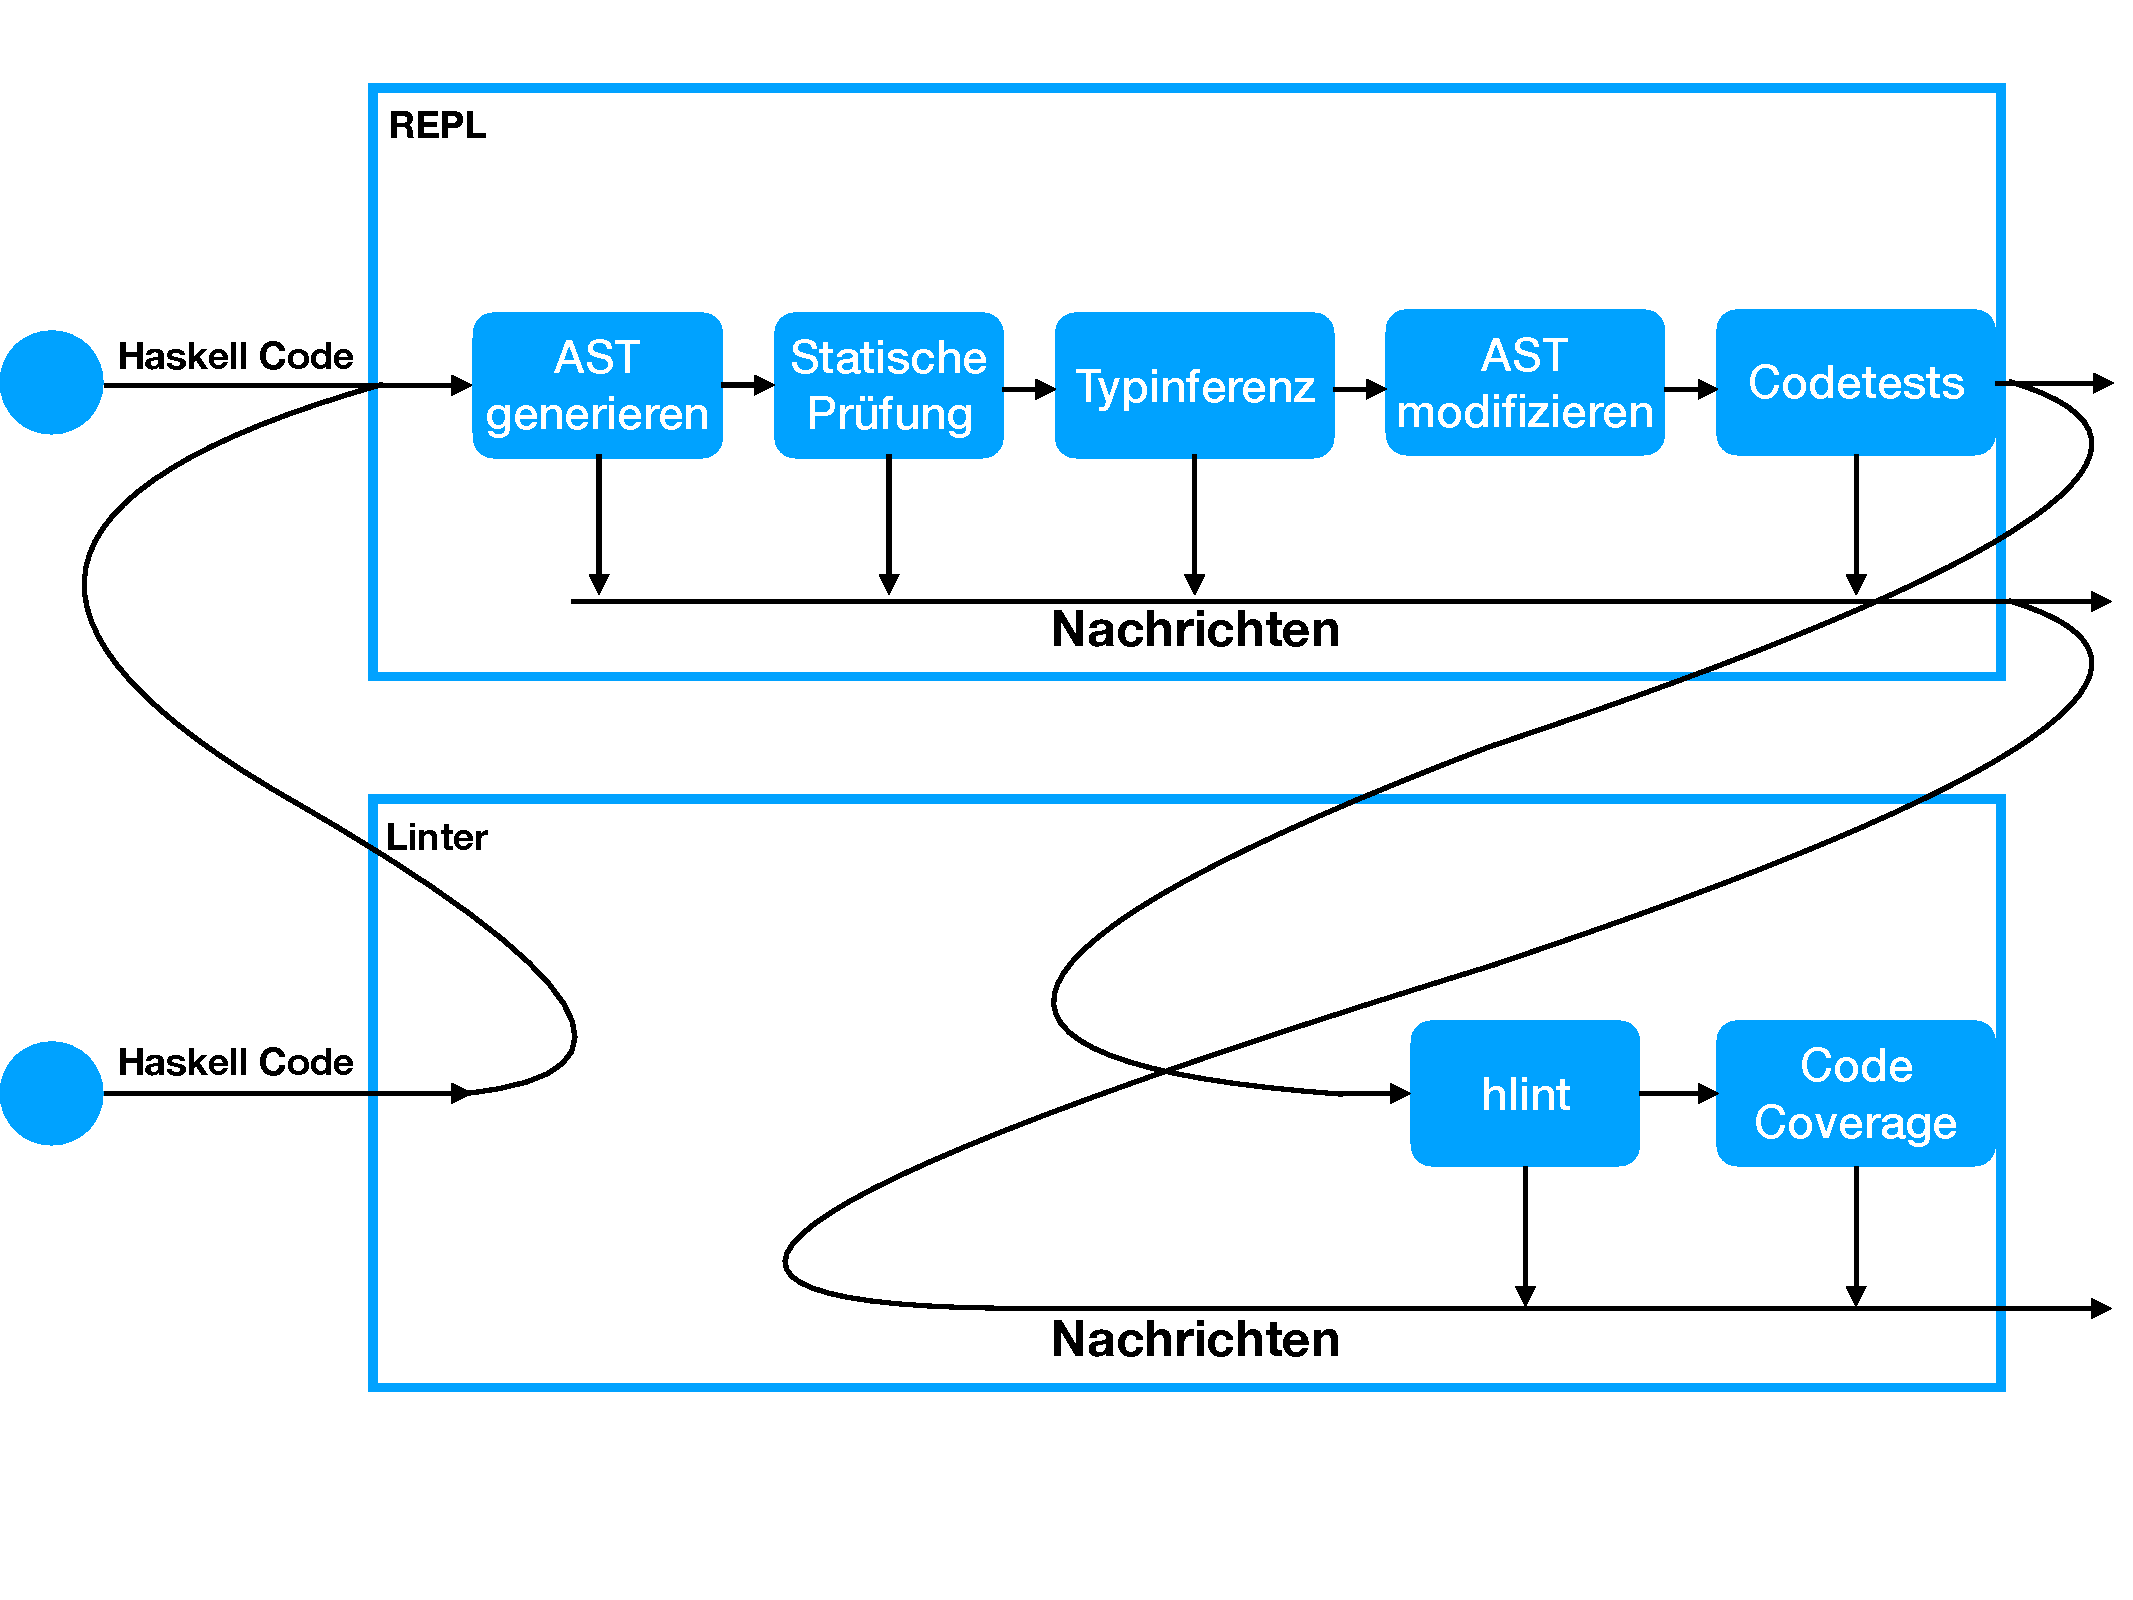
\includegraphics[width=1.0\textwidth, angle=0]{architecture.pdf}
\end{frame}
\begin{frame}
	\frametitle{Installation}
	\begin{itemize}[<+->]
		\item{Zwei Möglichkeiten}
		\item{Cabal}
			\begin{enumerate}
				\item{Klonen des Git-Repositorys}
				\item{cabal sandbox init}
				\item{cabal install}
				\item{Direktes Aufrufen der Programme aus der Cabal-Sandbox}
			\end{enumerate}
		\item{Docker}
			\begin{enumerate}
				\item{docker pull jonasbusse/drhaskell}
				\item{Benutzung über vorgefertigte DockerCall-Skript}
			\end{enumerate}
	\end{itemize}
\end{frame}
\begin{frame}
	\frametitle{Fazit}
	\begin{itemize}[<+->]
		\item{Erweiterbare REPL mit eigener Typinferenz und Testrunner}
		\item{Erweiterbares Stufensystem}
		\item{Ausführen statischer Check vor dem Laden}
		\item{Leichter verständliche Fehlermeldungen durch Einschränkung der Möglichkeiten}
		\item{Einfaches Schreiben von Testfällen}
		\item{Linter mit CodeCoverage-Anzeige der Testfälle}
		\item{Untersützt den Benutzer beim Lernen von Haskell}
	\end{itemize}
\end{frame}
\begin{frame}
	\frametitle{Ausblick}
	\begin{itemize}[<+->]
		\item{Typinferenz mit Typklassen}
		\item{Vorbedingungen für CheckExpect-Syntax}
		\item{Benutzerdefinierte Levelkonfiguration}
	\end{itemize}
\end{frame}
\end{document}


